%--------------------------------------
% Create title frame
\titleframe

\begin{frame}{Access to the course material}
    \centering
    \alert{\url{https://github.com/bcornelusse/DENSYS-school}}\\[2mm]
    
\includegraphics[width=0.3\textwidth]{frame.png}
\end{frame}


%--------------------------------------
% Table of contents
\begin{frame}{Overview}
  \setbeamertemplate{section in toc}[sections numbered]
  \tableofcontents[hideallsubsections]
\end{frame}


%==============================================
\section{Introduction}
%==============================================
\begin{frame}{Goal of the week}
\centering 
\begin{minipage}{0.7\textwidth}
\large Apply optimization and machine learning to microgrid optimal control, optimal design, and forecasting.
\end{minipage}
\end{frame}

\begin{frame}{The objectives are for you to learn to}
\begin{itemize}
    \item Model and optimize a microgrid (without the electrical grid) 
    \item Build power and energy management systems
    \item Make some forecasts of electricity generation and consumption
    \item Apply optimization
    \item Apply machine learning
    \item Code in Python
\end{itemize}
\end{frame}


%==============================================
\section{Microgrids and distribution networks}
%==============================================


\begin{frame}{Microgrids}

\begin{block}{A microgrid definition}
A  small electrical network composed of decentralized energy resources, loads, and energy storage devices. It is controlled and operated locally. It can connect or disconnect from the main grid.
\end{block}
\end{frame}

\begin{frame}{Schematic representation of a microgrid}
\centering
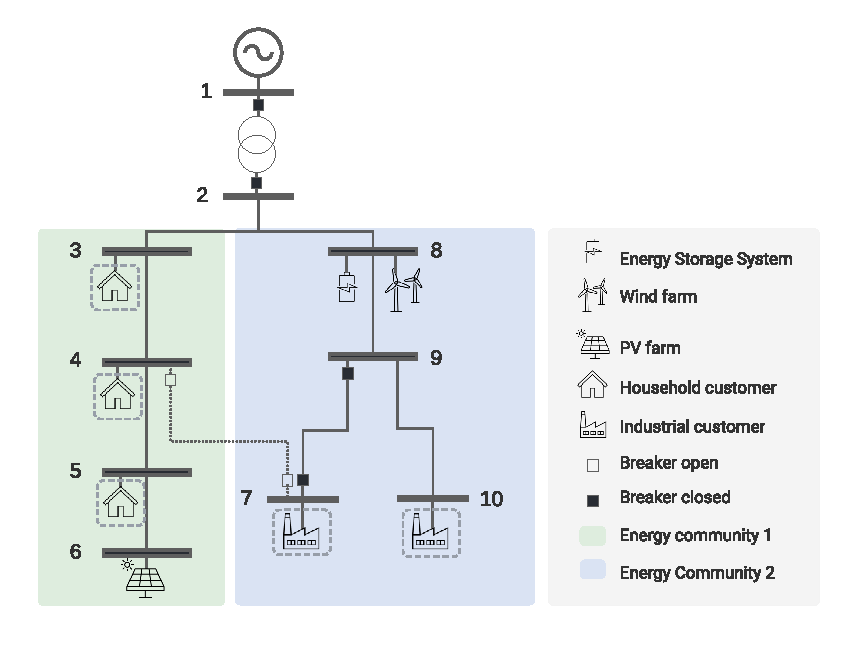
\includegraphics[width=0.6\textwidth]{distrib.pdf}
\end{frame}

\begin{frame}{Behind a connection point}
\centering
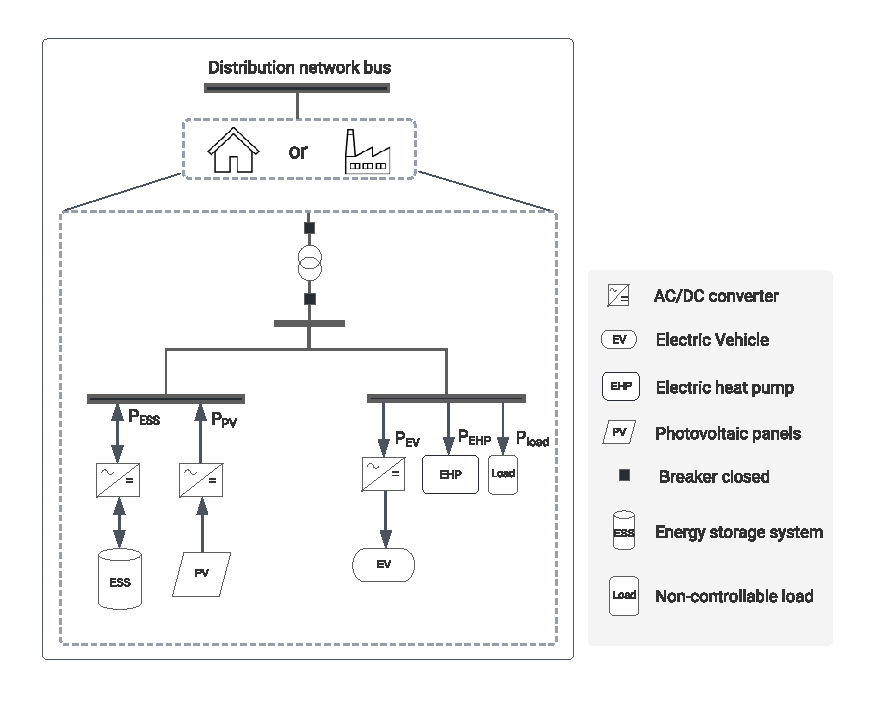
\includegraphics[width=0.6\textwidth]{grid_user.pdf}
\end{frame}

\begin{frame}{Temporal dimension: photovoltaic generation}
\centering
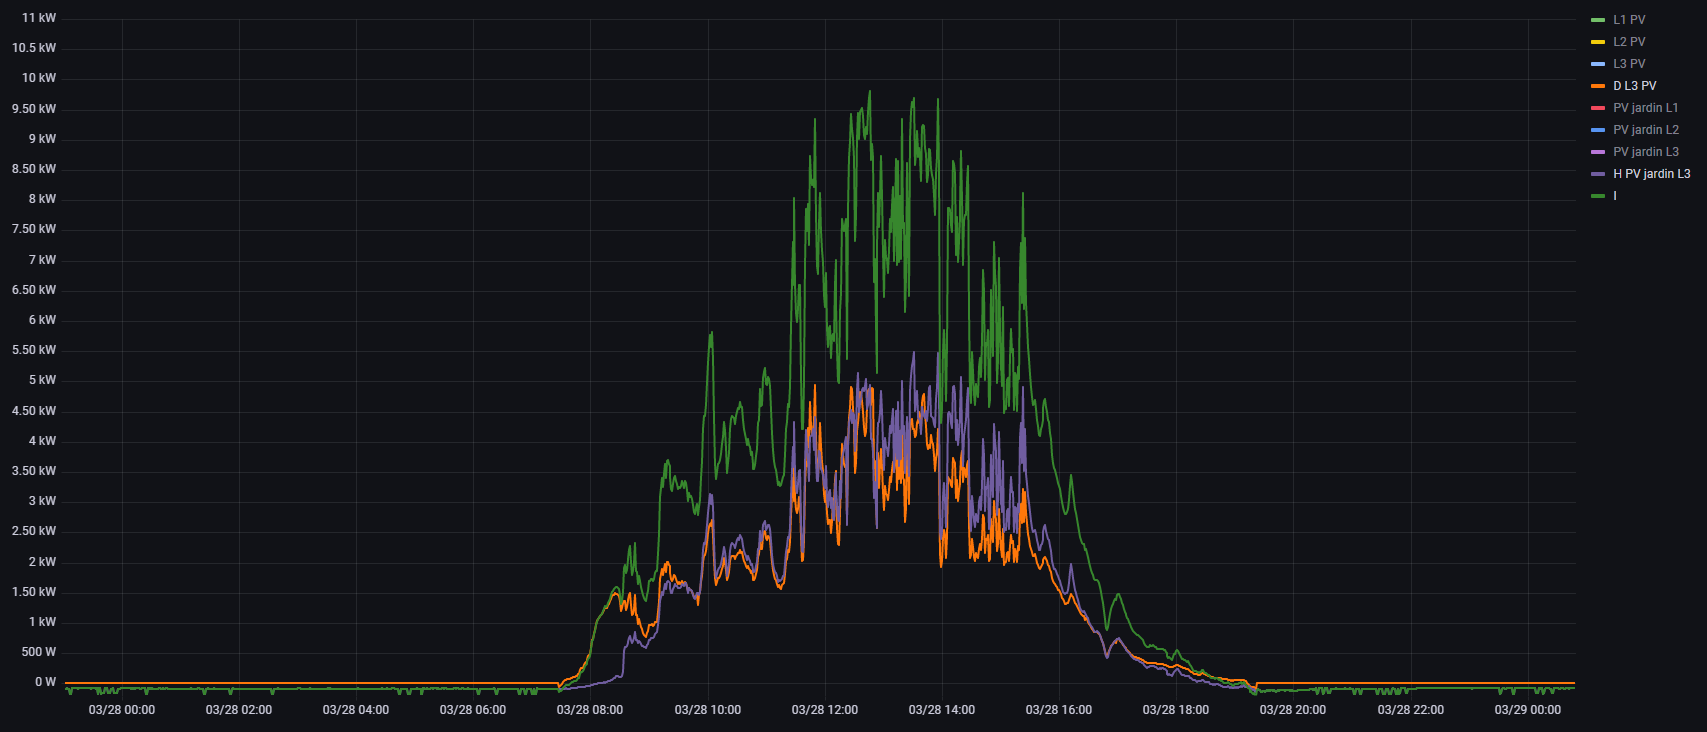
\includegraphics[width=\textwidth]{PV.png}
\end{frame}

%==============================================
\section{Microgrid control levels}
%==============================================

\begin{frame}{Microgrid controller}


\begin{block}{Microgrid controller}
Software that senses the microgrid (currents, voltages, frequency, etc.) and takes control actions to operate the microgrid safely, reliably, and optimally.
\end{block}

In practice, a microgrid is run by multiple controllers because there are several levels of control, which differ by their spatial and temporal scopes.

Next to technological advances in production, consumption, and storage, controllers are crucial elements for advanced microgrids.
\end{frame}

\begin{frame}{The four control levels in a microgrid}
 \begin{table}[H]
    \centering
    \caption{The four control levels}
    \begin{tabular}{@{} rl @{}}
	\toprule
	\textbf{Level} & \textbf{Function} \\
        \midrule
	1 & Device level control \\
	2 & Local area control \\
	3 & Supervisory control \\
	4 & Public grid interaction \\
      \bottomrule
    \end{tabular}
\end{table}
\end{frame}

\begin{frame}{Level 1: device level control}
\begin{itemize}
\item Generator control
\item PV panel + MPPT + inverter
\item A great variety of interfaces for loads
\item Battery storage: battery management system (BMS)
\item Battery inverter/charger
\item Islanding detection: Automatic transfer switch
\end{itemize}
\end{frame}

\begin{frame}{Level 2: local area control}
\begin{itemize}
\item Fast, automatic load/generation control to ensure constant balance and
  achieve stable operating points:
  \begin{itemize}
  \item regulate active and reactive power in AC microgrids
  \item achieving stable operation may be a challenging problem because of the:
    \begin{itemize}
    \item dynamic response mismatches between loads and sources,
    \item generated power capacity close to the nominal load,
    \item reduced added energy storage in generator rotors (if any).
    \end{itemize}
  \end{itemize}
\item (Unplanned) disconnection management
\item Resynchronization
\end{itemize}
\end{frame}

\begin{frame}{Level 3: supervisory control}
\begin{itemize}
\item Generation and load dispatch
\item Economic optimization
\item Spinning reserve
\item Forecasting
\item Data visualization and data management
\end{itemize}
\end{frame}

\begin{frame}{Level 4: public grid interaction}

\begin{itemize}
\item Distribution Management System interaction
\item Electricity markets
\item Ancillary services markets
\end{itemize}
\end{frame}

%\begin{frame}[allowframebreaks]{References}
%  \bibliography{demo}
%  \bibliographystyle{abbrv}
%\end{frame}